\chapter{結果と評価}
\label{chap:results}
本章では,3章で紹介した手法によって自動生成した吹奏アニメーションについて記述する.
\secref{sec:system}では仕様したPCやシステムの仕様を述べ,
\secref{sec:result}では自動生成した吹奏アニメーションのキャプチャリング画像を示す.
そして\secref{sec:review}では自動生成結果を実際の演奏シーンや既存の吹奏アニメーションと比較することにより,提案手法を評価する.

\section{実行環境} \label{sec:system}
事前にUnreal Engineにて専用のプロジェクトを作成し,モーションのデータが記載されているUnreal Engine専用のファイルをインポートする.
そして,キャラクタと,それぞれが演奏する楽器を\figref{fig:ue4}のようにセッティングする.
なお,最初にインポートするUnreal Engine専用のファイルには,キャラクタの姿勢データも存在するため,
キャラクタの姿勢のセッティングは容易にできる.\\
\indent
実行環境は\tabref{tab:pc}の通りである.
\begin{figure}[h]
	\centering
	\includegraphics[width=14cm]{fig/chap4/ue4.eps}
	\caption{Unreal Engineの初期設定}
	\label{fig:ue4}
\end{figure}

\begin{table}[htbp] 
	\begin{center}
		\caption{実行環境}
		\label{tab:pc}
		\begin{tabular}{|l|c|}
			\hline
			OS & Windows10 64bit \\ \hline
			CPU & Intel\textregistered Core\textsuperscript{TM}i7-3930K \\ \hline
			RAM & 32.00GB\\ \hline
			言語 & c++\\ \hline
		\end{tabular}
	\end{center}
\end{table}

\section{アニメーション生成結果} \label{sec:result}
本研究で作成したアニメーションは,主に少人数編成であるアンサンブルアニメーションである.
以下では,トランペット奏者2名で演奏するアニメーションのキャプチャリング画像と,
トランペット奏者2名,トロンボーン奏者2名の計4名で演奏するアニメーションのキャプチャリング画像を示す.
以下,それぞれについて制御している口元やボーンの制御について説明するが,
前者のアニメーションは口元や指元がズームインされているシーンであるため,主に口元や指元のボーンの制御について,
後者のアニメーションは全体を俯瞰しているシーンであるため,主に指元以外のボーンの制御について述べる.\\
\indent
\figref{anim1}は,トランペット奏者2名の基本姿勢である.
\begin{figure}[h]
	\centering
	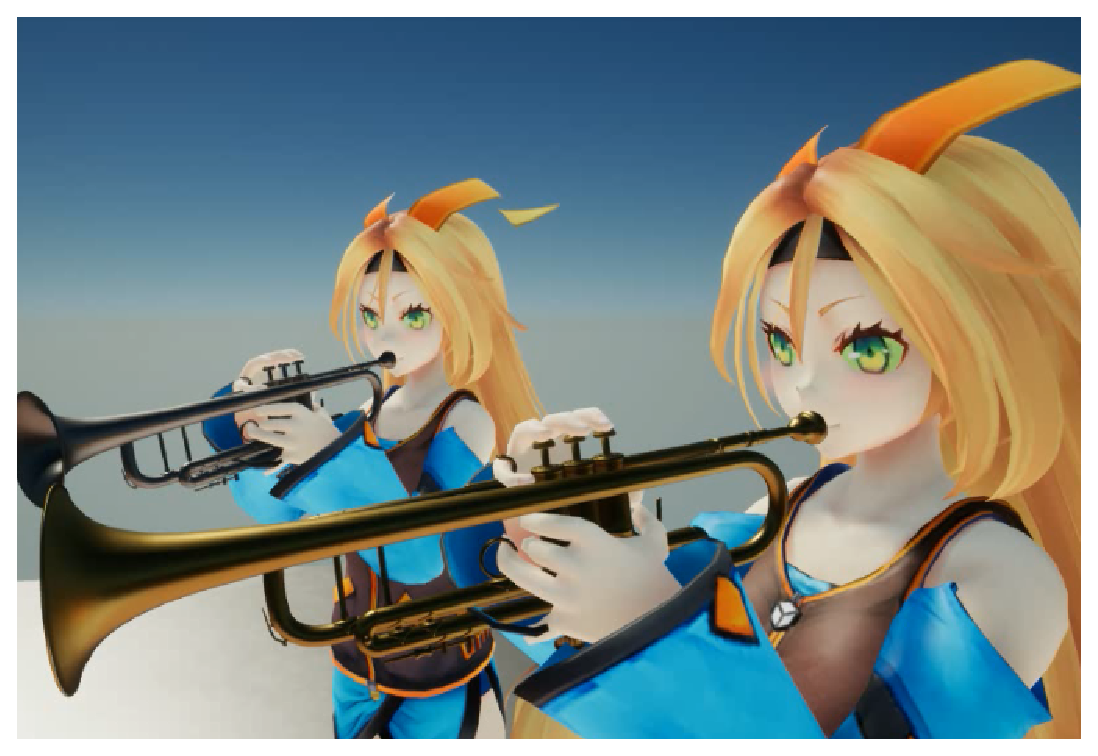
\includegraphics[width=10cm]{fig/chap4/anim1.eps}
	\caption{トランペット奏者2名の基本姿勢}
	\label{fig:anim1}
\end{figure}
音を鳴らすタイミングで,演奏者は\figref{anim1_finger}のように,指でトランペットのピストンを押す動作をする.
\begin{figure}[h]
	\centering
	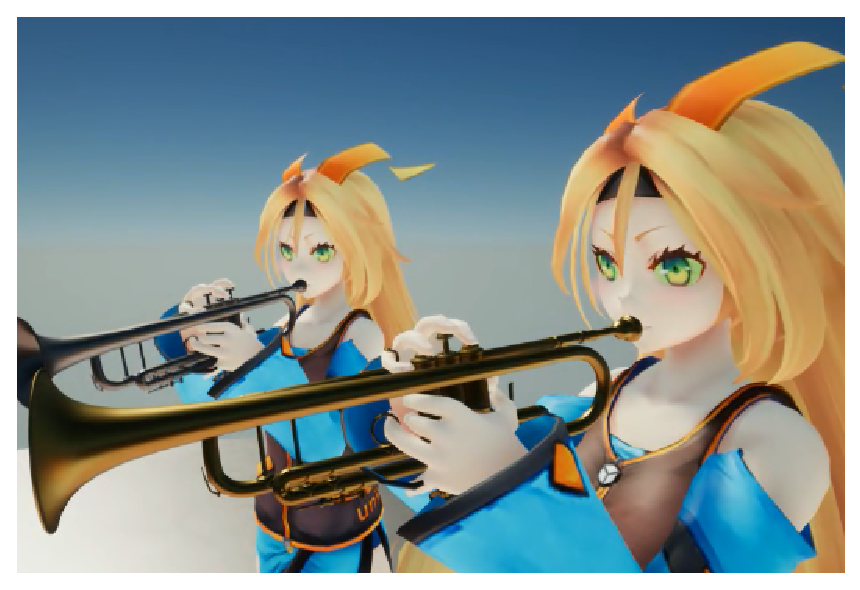
\includegraphics[width=10cm]{fig/chap4/anim1_finger.eps}
	\caption{トランペット奏者2名がピストンを押す姿勢}
	\label{fig:anim1_finger}
\end{figure}


\section{評価} \label{sec:review}

\subsection{実際の演奏シーンとの比較による評価}

\begin{figure}[t]
	\centering
	\subcaptionbox{\textgt{吹奏楽・オーケストラ経験者の回答}
		\label{fig:unity}}[0.75\linewidth]{
		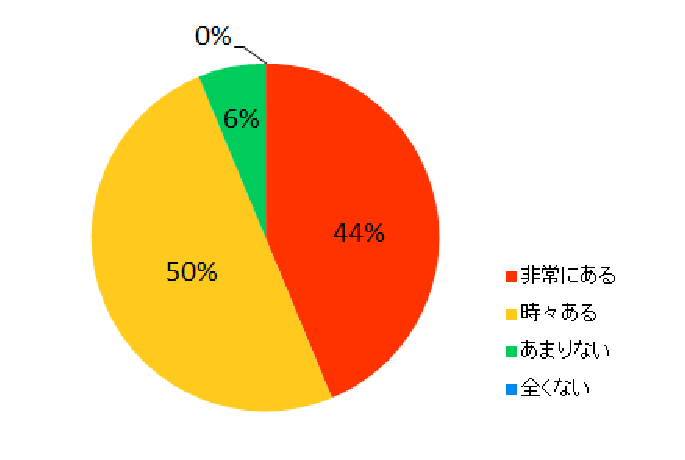
\includegraphics[height=7cm]{fig/chap1/Q1-1.eps}}
	\subcaptionbox{\textgt{吹奏楽・オーケストラ未経験者の回答}
		\label{fig:tp}}[0.6\linewidth]{
		\includegraphics[height=5.5cm]{fig/chap1/Q1-2.eps}}
	\caption{演奏アニメーションが不自然であると感じることがあるかどうか}
	\label{fig:model}
\end{figure}

\subsection{既存のアニメーションとの比較による評価}

\subsection{アンサンブルアニメーションの評価}

\subsection{システムの有用性の予想}